\section{The RobWork library and its functionalities}
\label{sec:RW_lib_and_func}
This chapter is a general introduction to the RobWork library and the most commonly used data structures and functionalities within. There is a lot more to RobWork than what is in this chapter, the point of this chapter is to give a intuitive understanding of the RobWork library. More information about RobWork can be found on official homepage for the RobWork project \cite{RW_Webpage}.


\subsection{WorkCells}
A WorkCell is the basis structure in RobWork. The WorkCell can be thought of as a box containing all of the other building blocks and information needed to represent an environment (See figure~\ref{fig:WorkCellBoxExample}). The WorkCell most commonly contains Frames, Objects, Devices which are used to represent the different items in the environment. The WorkCell also contains a State Structure used to describe how the items in the environment are related. The WorkCell also contains collision information for the environment.

\begin{figure}[h]
	\centering
	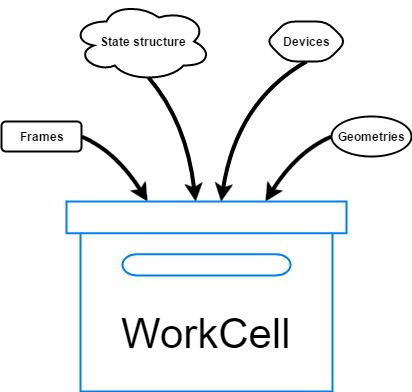
\includegraphics[scale=0.55]{Figures/WorkCellBoxExample.png}
	\caption{The WorkCell can be seen as a box containing the elements necessary to represent an environment}
	\label{fig:WorkCellBoxExample}
\end{figure}


\subsection{Frames}
One of the most common data structures from the RobWork library is a frame. A frame is the basic building block in the RobWork library, representing (in the case of RobWork) a local 3D euclidean space. In RobWork frames are built in sequence to each other to form the environment. This means that all frames have a parent and potentially children.\\

In RobWork frames come in 3 different types: fixed frames, moveable frames and joints.\\
Fixed frames are frames that have a constant transform relative to the parent frame.\\
Movable frames are frames which transform can be freely changed.\\
Joints are frames that can be assigned values for position, velocity limits and acceleration limits. This type of frame is usually used for devices. Joints can be further divided into 3 subtypes: prismatic joint, revolute joint and dependent joint.\\
Prismatic joints are joints which motion is linear along a constant direction. Thinking of a pneumatic piston can be an intuitive way of thinking about prismatic joints.\\
Revolute joints are joints which motion is based on a rotation around a single axis. Thinking of hinges can be an intuitive way of thinking about revolute frames.\\
Dependent joins refer to joints which transform depends on one or multiple other joints. Dependant joins can also be divided into 2 subtypes, dependent prismatic joints and dependent revolute joints, adding the motion specification of the prismatic joint and revolute joint previously mentioned.\\

Frames in a WorkCell are required to have a parent and are given a unique name so that no frames can be confused for another. Only one frame in the WorkCell has no parent. This frame is called WORLD and is created when the WorkCell is constructed. The WORLD frame can be seen as the global 3D euclidean space for the WorkCell.

In RobWork there is also a special kind of frame called a DAF frame. DAF stands for dynamically attachable frame. A DAF frame is a frame which is implemented so that the parent of the frame is more dynamic to change.

\subsection{Objects}
Contrary to frames which represents the relationships in the environment, objects represents physical things in the scene. Also contrary to frames is that the name of an object does not have to be unique.\\

In order for objects to get a relationship to the environment it is placed in, it has to be associated to a frame. This frame is called the base frame of the object. An object can be associated to multiple frames but only have one base frame.\\

An object consists of two important elements, a geometry and a model.\\
A geometry is used to represent the actual geometry of the object. The geometry can be scaled and transformed to allow for modifications. In order to perform a transform, the geometry need a reference. This is done with having the reference be a frame, a reference frame. RobWork is capable of creating simple geometries like spheres, boxes and cylinders, however it is also possible to import complex geometries. Geometries are also being used for the collision detection provided in RobWork.\\
A model is a graphical representation of the object. Models consists of geometries, materials, colors and texture information as well. It is also possible to apply a transform to a model and get the transform of a model.\\
Usually when an object is created, a geometry is created for collision detection and a model is created to visually represent the object in a viewer(e.g. RobWorkStudio).\\

There are two types of objects in RobWork, rigid objects and deformable objects. Rigid objects are objects which  geometry does not change. Rigid objects can also posses information about inertia and mass. A deformable object however has the ability to alter its geometry via control nodes.


\subsection{Devices}
A device can be considered a description of a arbitrary device e.g. the FANUC LRM200 robotic arm (Seen on figure~\ref{fig:FANUCLRM200}). The device also contains the configurations for the device it represents. These configurations are contained in a single configuration vector, making it easy to control the device. In case of a joint device (like the FANUC LRM200), it is also possible to get and set the bounds, velocity limits and acceleration limits for the joints.\\

\begin{figure}[h]
	\centering
	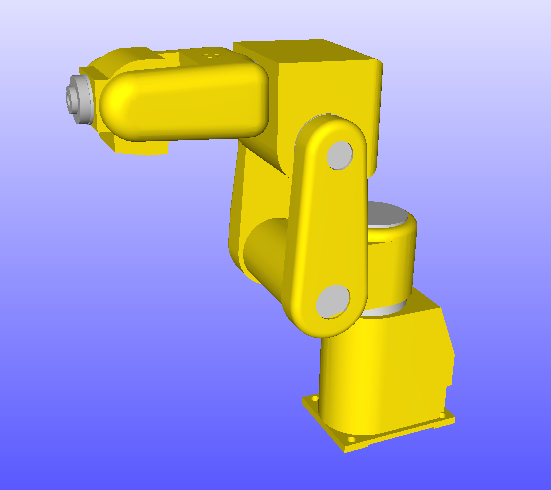
\includegraphics[scale=0.55]{Figures/FANUCLRM200.png}
	\caption{Model of a FANUC LRM200 in RobWorkStudio}
	\label{fig:FANUCLRM200}
\end{figure}

Devices can be of 3 different types: joint device, mobile device and SE3 device. Mobile devices are devices that  is differentially controlled e.g. a robot rover. Joint devices are devices that consists of moving joints much like the previously mentioned FANUC LRM200 robotic arm. SE3 devices are devices that can move in a 3D euclidean space and is not consisting of joints e.g. a drone.\\

Joint devices can be of 5 types: Serial devices, tree devices, parallel devices, composite devices and composite joint devices.\\
Serial devices are the simplest form of device since it consist of joints set in serial to each other. Many simple robotic arms like the before mentioned FANUC LRM200 are serial devices.\\
Tree devices are devices which joints follow a tree structure, meaning that a joint can have multiple children but only one parent joint. This also means that a tree device must have more than one end effectors. This type of device is typically seen in dexterous hands.\\
Parallel devices are devices that at some point in the structure, of the device, is created a circle e.g. a joint goes to two joints that then both go to the same joint. The two middle joints are said to be in parallel to each other and are called parallel legs in RobWork. Parallel legs can consist of multiple joints as well as just one.\\
Composite devices and composite joint devices are devices that are constructed from a series of other devices. The devices in the composite device may not share joints. Just like tree devices, composite devices can have multiple end effectors. However unlike the tree devices, composite devices does not require the path to the end effectors to have a common base. The difference between composite devices and composite joint device is that the devices used in a composite joint device needs to be of the joint device type, whereas in a composite device this is not a requirement.\\
Illustrations of the joint device types can be seen on figure~\ref{fig:DeviceTypes}.

\begin{figure}[h]
	\centering
	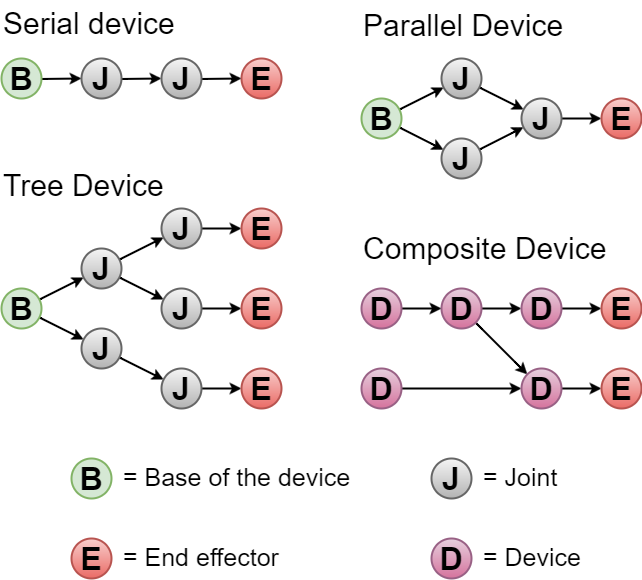
\includegraphics[scale=0.55]{Figures/DeviceTypes.png}
	\caption{The WorkCell can be seen as a box containing the elements necessary to represent an environment}
	\label{fig:DeviceTypes}
\end{figure}

\subsection{3D Transforms}
In the RobWork library the general way of moving around frames and other items is through the concept of transforms. For application regarding a 3D euclidean space, it is normal to use 3D transforms. A 3D transform is a 4 by 4 matrix. This matrix is created from a 3 element vector containing the displacement and a 3 by 3 matrix containing the rotation. In RobWork, the rotation is commonly given in roll, pitch and yaw values, which is a way to describe the rotation with 3 values instead of the 3 by 3 matrix. Roll, pitch and yaw is normally refered to as the RPY or R, P, Y values. On figure~\ref{fig:RPYExample} is an illustration of what the RPY values represent using a plane.

\begin{figure}[h]
	\centering
	\includegraphics[scale=0.55]{Figures/RPYExample.png}
	\caption{Illustration of the RPY values using a plane \cite{RPY}}
	\label{fig:RPYExample}
\end{figure}

\subsection{States and State Structures}
In RobWork the structure of the frames are represented through a class called State Structure. The State Structure also holds the state of all the frames in the form of a class called State. The State is a collection of the states of all the frames contained in the State Structure. This is done as a kinematic tree.


\subsection{Namespacing in RobWork}
The RobWork library is neatly divided into sections. Some of the more used sections are kinematics, models, geometry, loaders and math. When writing code using the RobWork library the namespace of the class one would want to access is the same as division of the library. As an example, accessing the the frame class from the kinematics section would be done like rw::kinematics::Frame. This makes it easier to locate the implementation of a class or fuctionality e.g. the implementation of the frame class is in the kinematics folder.\\

Most of the functionalities in RobWork are implemented as static functions. This makes coding with the RobWork library more intuitive since for some of the functionalities in RobWork it does not make sense to require an object to access the functionalities. As an example, accessing the load function of the XMLRWLoader (which loads in a XML-file describing the WorkCell) can be done simple by writing rw::loaders::XMLRWLoader::load(input for function), instead of creating a object of the XMLRWLoader and then calling load on the object.


\subsection{Typical use of RobWorkStudio and WorkCell-files}
Typically when using RobWorkStudio, the user create a WorkCell file written in XML. This file contains the necessary information for creating a WorkCell. The WorkCell file can then be loaded into RobWorkStudio by using the open button. The WorkCell file can also be loaded manually with the before mentioned XMLRWLoader returning a WorkCell object. When creating a WorkCell file it is necessary to know the tags used by RobWork. The root element in a WorkCell file is the WorkCell tag. The WorkCell tag should be written with the attribute name, giving the WorkCell a name. Inside the WorkCell tag different tags can be used to add the elements of the WorkCell. Some of the more common tags used are: frame, RPY, pos, joint, geometry tags, device tags and the include tag.\\
The frame tag is used to define a frame in the structure. The frame tag needs to be supplied with a name attribute and a type attribute defining the frame type.\\
The RPY tag is used within the frame tag to define the rotation of the frame and the pos tag is used to define the displacement. A transform can be used instead of these if the transform is available.\\
The joint tag is representing a frame of the type joint. This tag also needs a name attribute and a type attribute to define the type of joint.\\
There are also some simple geometry tags that are used for define simple geometries like a box. More complex geometries can be included via a polytype tag taking in the path for the model file.\\
Devices can be defined using different tags that define the different kind of devices in RobWork. As an example the serial device FANUC LRM200 would have a serial device tag with joint tags inside.\\
The include tag is used to include another XML file's content. This is usually used to include complex devices into an environment. This allows users to create only one description of a device and then include it whenever it is used. An example of a WorkCell described in XML can be seen in figure~\ref{fig:XMLCodeExample}.

\begin{figure}[h]
\centering
\lstset{language=XML} 
\begin{lstlisting}[frame=single]
<!-- WorkCell with the name attribute set to Scene -->
<WorkCell name="Scene"> 

<!-- New Frame called Table added to the World frame -->
  <Frame name="Table" refframe="WORLD" >
	<!-- Transform of the Table frame -->
    <RPY>0 0 0</RPY><Pos>0.2 0.2 -0.408</Pos> 
  </Frame>
  
<!-- New model named Table added to the Table Frame -->
  <Drawable name="Table" refframe="Table" >
	<!-- Transform of the model Table -->
    <RPY> 0 0 0</RPY> <Pos> 0 0 0 </Pos>
	<!-- Model information (box) of the model -->
    <Box x="0.8" y="0.8" z="0.816" />
  </Drawable>

<!-- New Frame called URMount is added to the frame Table -->
  <Frame name="URMount">
	<!-- Transform of the URMount frame -->
    <RPY>90 0 0</RPY><Pos>0 0 0</Pos> 
  </Frame>
  
<!-- Include the UR robotic arm from another xml file -->
  <Include file="../../XMLDevices/UR-6-85-5-A/UR.wc.xml" />	

</WorkCell>			 
\end{lstlisting}
\caption{Example of a WorkCell written in XML containing a UR robotic arm on a table. This example is from the examples following the the RobWork library (ModelData/XMLScenes/RobotOnTable)}
\label{fig:XMLCodeExample} 	
\end{figure}

